% Binomial-probability.tex
% Topic: Binomial Probability

A \textbf{binomial experiment} has the following properties:
\begin{itemize}[leftmargin=*]
  \item A fixed number $n$ of trials.
  \item Each trial has exactly two outcomes: \textit{success} or \textit{failure}.
  \item The probability of success $p$ is the same on every trial.
  \item The trials are independent.
\end{itemize}

If $X$ is the number of successes in $n$ independent trials with probability $p$ of success, then
\[
P(X = r) = \binom{n}{r}\,p^r\,(1-p)^{n-r}, \qquad r = 0, 1, 2, \ldots, n.
\]

\textbf{Cumulative binomial probability:}
\[
P(X \leq k) = \sum_{r=0}^{k} \binom{n}{r}\,p^r\,(1-p)^{n-r}.
\]

\begin{center}
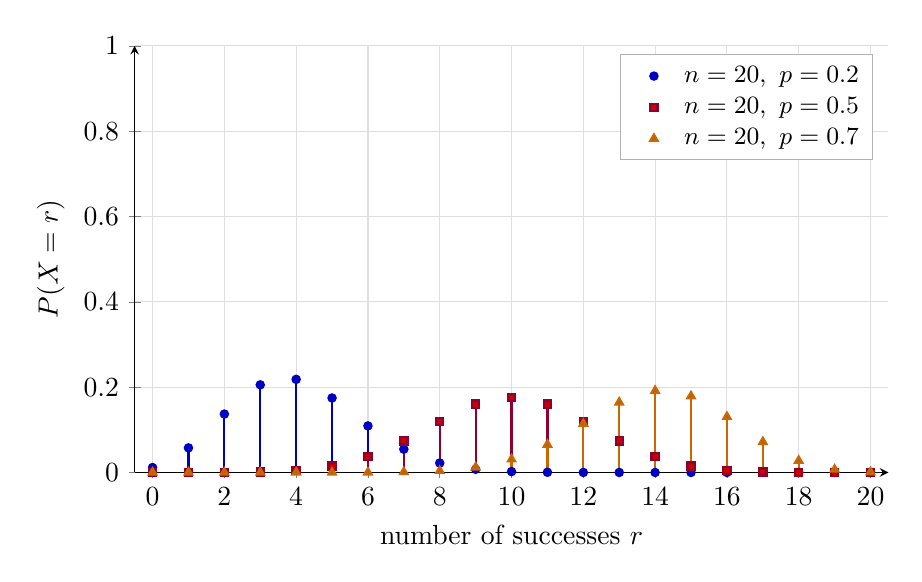
\begin{tikzpicture}
\begin{axis}[
    width=0.92\textwidth,
    height=7cm,
    xmin=-0.5, xmax=20.5,
    ymin=0, ymax=1,
    axis lines=left,
    xlabel={number of successes $r$},
    ylabel={$P(X=r)$},
    xtick={0,2,4,6,8,10,12,14,16,18,20},
    ytick={0,0.2,0.4,0.6,0.8,1.0},
    grid=both,
    major grid style={gray!25},
    minor grid style={gray!10},
    legend style={
      at={(0.98,0.98)},
      anchor=north east,
      draw=gray!60,
      fill=white,
      font=\small
    },
    legend cell align=left
]
\addplot+[ycomb, thick, mark=*, mark size=1.3pt, blue!75!black]
coordinates {
(0,0.011529) (1,0.057646) (2,0.136909) (3,0.205364) (4,0.218199)
(5,0.174560) (6,0.109100) (7,0.054550) (8,0.022161) (9,0.007387)
(10,0.002031) (11,0.000462) (12,0.000087) (13,0.000013) (14,0.000002)
(15,0.000000) (16,0.000000) (17,0.000000) (18,0.000000) (19,0.000000)
(20,0.000000)
};
\addlegendentry{$n=20,\ p=0.2$}

\addplot+[ycomb, thick, mark=square*, mark size=1.3pt, purple!75!black]
coordinates {
(0,0.000001) (1,0.000019) (2,0.000181) (3,0.001087) (4,0.004621)
(5,0.014786) (6,0.036964) (7,0.073929) (8,0.120134) (9,0.160179)
(10,0.176197) (11,0.160179) (12,0.120134) (13,0.073929) (14,0.036964)
(15,0.014786) (16,0.004621) (17,0.001087) (18,0.000181) (19,0.000019)
(20,0.000001)
};
\addlegendentry{$n=20,\ p=0.5$}

\addplot+[ycomb, thick, mark=triangle*, mark size=1.5pt, orange!80!black]
coordinates {
(0,0.000000) (1,0.000000) (2,0.000000) (3,0.000001) (4,0.000005)
(5,0.000037) (6,0.000218) (7,0.001018) (8,0.003859) (9,0.012007)
(10,0.030817) (11,0.065370) (12,0.114397) (13,0.164262) (14,0.191639)
(15,0.178863) (16,0.130421) (17,0.071604) (18,0.027846) (19,0.006839)
(20,0.000798)
};
\addlegendentry{$n=20,\ p=0.7$}
\end{axis}
\end{tikzpicture}
\end{center}
\noindent\textit{Figure: binomial probability mass functions for $X\sim B(20,p)$. As $p$ increases, the distribution shifts to the right because the expected number of successes is $np$.}
